\documentclass{beamer}

\usepackage{beamerthemesplit}
\usepackage{amsmath}
\usepackage{amsfonts}
\usepackage{amssymb}
\usepackage{qtree}
\usepackage{cancel}
\usepackage{tkz-graph}
%\usepackage[pdftex]{graphicx}

\mode<presentation>
{
  \usetheme{Warsaw}
  % or ...

  %\setbeamercovered{transparent}
  % or whatever (possibly just delete it)
}


\usepackage[english]{babel}
% or whatever

\usepackage[latin1]{inputenc}
% or whatever

\usepackage{times}
\usepackage[T1]{fontenc}

\title{Automated Program Learning}

\subtitle{MOSES}

\author{Nil Geisweiller}

\institute[Xiamen University] % (optional, but mostly needed)
{
  Novamente LLC
}

\date[Xiamen University AGI Summer School 2009] % (optional, should be abbreviation of conference name)
{Xiamen University\\ AGI Summer School 2009}


\AtBeginSection[]
{
  \begin{frame}<beamer>{Outline}
    \tableofcontents[currentsection,currentsection]
  \end{frame}
}

\AtBeginSubsection[]
{
  \begin{frame}<beamer>{Outline}
    \tableofcontents[currentsection,currentsubsection]
  \end{frame}
}

%\newcommand{\AND}{\textit{AND}}
%\newcommand{\OR}{\textit{OR}}
%\newcommand{\NOT}{\textit{NOT}}
\newcommand{\AND}{\land}
\newcommand{\OR}{\lor}
\newcommand{\NOT}{\lnot}


\begin{document}

\frame
{
  \maketitle
}
\section[Outline]{}
\frame{\tableofcontents}

\section{Introduction}

\frame
{
  \frametitle{What is MOSES?}
  
  MOSES (\emph{Meta-Optimizing Semantic Evolutionary Search})
  Evolutionary program learning, PhD Moshe Looks.
  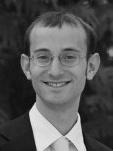
\includegraphics[scale=0.25]{moshe_head_bw.jpg}

  \begin{center}

  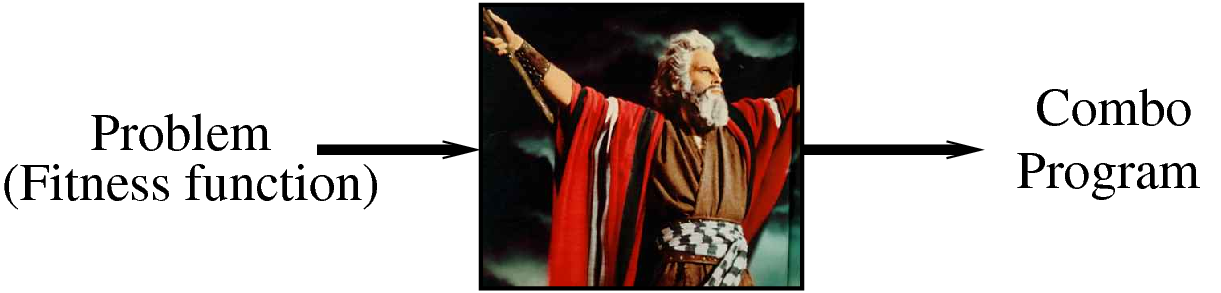
\includegraphics[scale=0.15]{MOSESSum2.png}

  \end{center}

  \begin{enumerate}
    \item<+-> Search programs that \alert{maximize the fitness} function
    \item<+-> Take advantage of \alert{program semantics}
      and program space topology
    \item<+-> Attempt to discover \alert{fitness landscape
        regularities to speed up the search}
    \end{enumerate}

}

\frame
{
  \frametitle{How it works?}

  \begin{center}

  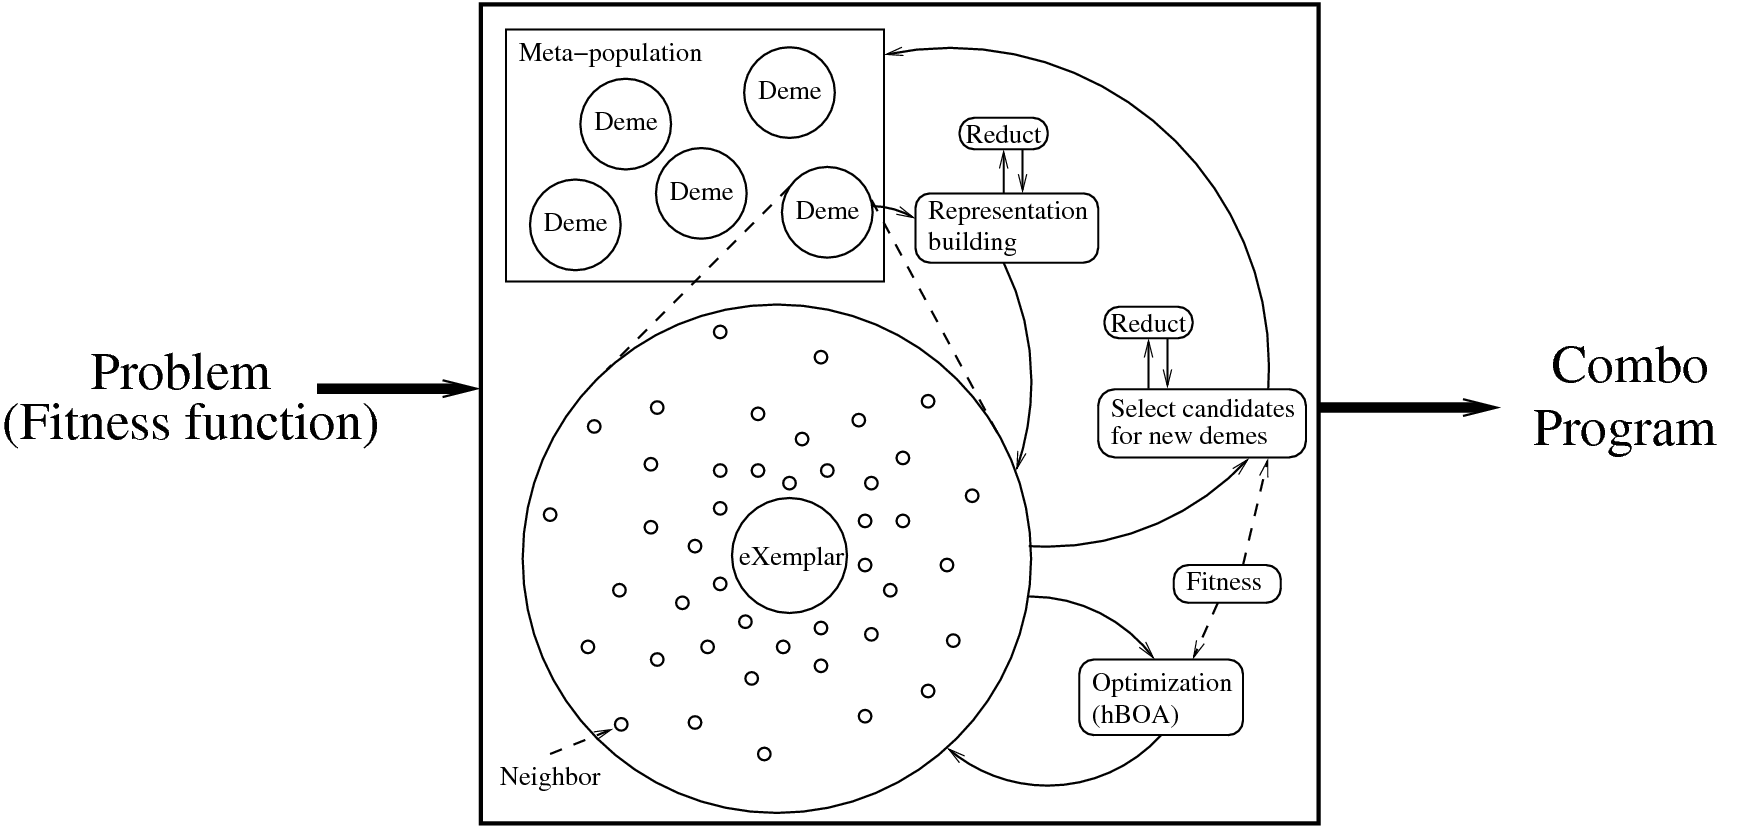
\includegraphics[scale=0.2]{MOSESSumDetails.png}

  \end{center}  

}

\frame
{

  \frametitle{How it works?}

  \begin{enumerate}
  \item<+-> Reduction in \alert{normal form}
    \begin{itemize}
    \item minimize over-representation
    \item improve syntactic vs semantic distance correlation
    \item simplify or even improve structure
    \end{itemize}
  \item<+-> Population building, \alert{representation-building}
    defines the \alert{deme's neighborhood}
  \item<+-> Optimization, find the best candidates in the deme's neighborhood.
    Learn how to \alert{differentiate good vs bad programs} and
    \alert{bias the search} accordingly
    \begin{itemize}
    \item hBOA
    \item Building-Block Hill Climbing (under development)
    \end{itemize}
  \item<+-> Deme management
    \begin{itemize}
    \item Set of demes, \alert{meta-population}
    \item Diversity, \alert{preserving interesting demes}
    \end{itemize}
  \end{enumerate}
}

\section{Representation-Building}

\frame
{
  \frametitle{Representation-building: Build a deme's population}

  \begin{center}

  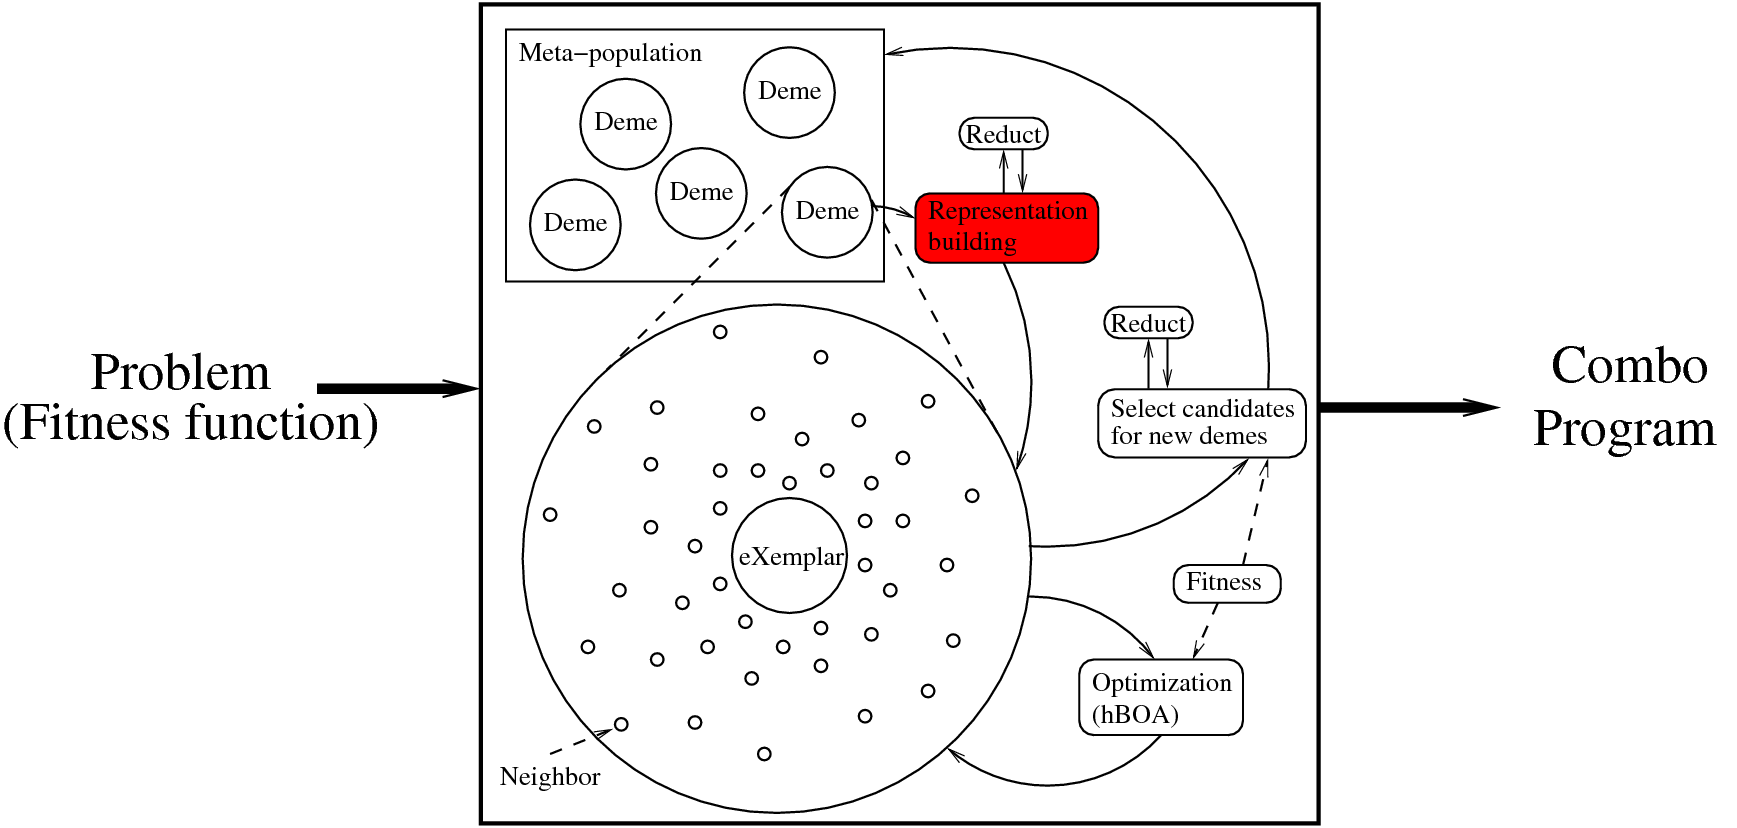
\includegraphics[scale=0.2]{MOSESSumDetailsRB.png}

  \end{center}  

}

\frame
{
  \frametitle{Building string of knobs}

  \begin{beamerboxesrounded}{Population of a Deme}
    \alert{Centered around an exemplar},
    each neighbor
    is a \alert{variation} of that exemplar according to the
    representation-building, a \alert{string of knobs}.
  \end{beamerboxesrounded}


  \begin{columns}
    
    \column{1.5in}
    {\tt and(\#1 not(\#2))}
    \column{0.2in}
    $\Rightarrow$
    \column{2in}
    
    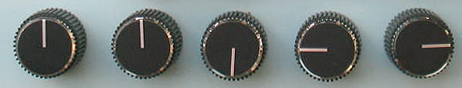
\includegraphics[scale=0.27]{knobs.png}
    
  \end{columns}
}

\frame
{
  \frametitle{Building string of knobs}
%  Exploiting
  Domain specific rules to create knobs,
%  knowledge for maximum expressivity
  example in the Boolean domain with {\tt and(x not(y))}:

  \begin{columns}

    \column{3in}
    
    \visible<+->{
      \begin{enumerate}[<+->]
      \item Under every junctor, $\forall$ $v$
        \alert{not already sibling},
        add [$\emptyset$, $v$, $not(v)$]
      \item Any junctor can be flipped
      \item Under every junctor
        add \alert{oposite junctor} + children
      \item Insert an \alert{oposite junctor} above the root + children
      \item And a few more...
      \end{enumerate}
    }
    \column{1in}

    \includegraphics[scale=0.2]<1,2>{build_knobs1.pdf}
    \includegraphics[scale=0.2]<3>{build_knobs2.pdf}
    \includegraphics[scale=0.2]<4>{build_knobs3.pdf}
    \includegraphics[scale=0.2]<5->{build_knobs4.pdf}
    
  \end{columns}

}

\frame
{
  \frametitle{Building string of knobs}

  \begin{center}
    \begin{figure}
      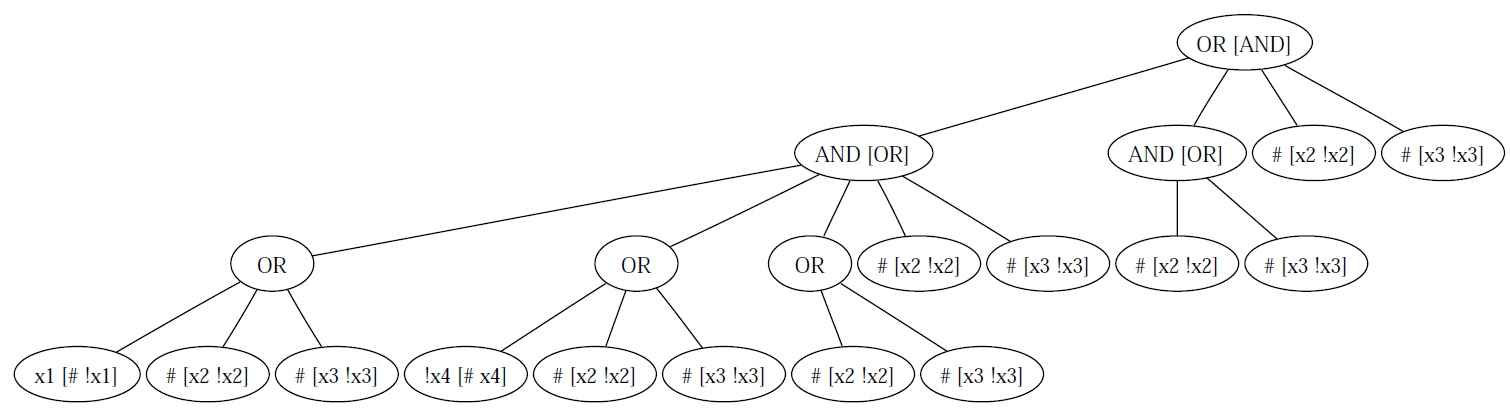
\includegraphics[scale=0.27]{knobs_building_example.png}
      \caption{Built knobs for \alert{$and(x_1 not(x_4))$},
        \emph{extracted from Moshe's PhD}.}
    \end{figure}
  \end{center}
}

\frame
{
  \frametitle{Optimization problem takes place on the knob string}

  \begin{center}
    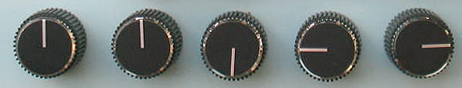
\includegraphics[scale=0.3]{knobs.png}
  \end{center}
%  ${\tt (and\ [or],\ \#\ [x\ not(x)],
%    \ \#\ [y\ not(y)], \#\ [x\ not(x)], \ \#\ [y\ not(y)])}$
%  \\
  For example:

  $
  \begin{array}{|c|c|c|}
    \hline
    {\text{knob setting}} & {\text{combo (reduced)}} & {\text{distance}}\\
    \hline
     {\tt (and,\ \emptyset,\ \emptyset,\ \emptyset,\ \emptyset)}
     &
     {\tt and(x\ not(y))}
     &
     0
     \\
    \hline
     {\tt (or,\ \emptyset,\ \emptyset,\ \emptyset,\ \emptyset)}
     &
     {\tt or(x\ not(y))}
     &
     1
     \\
     \hline
     {\tt (and,\ \emptyset,\ \emptyset,\ not(x),\ \emptyset)}
     &
     {\tt or(not(x)\ not(y))}
     &
     1
     \\
     \hline
     {\tt (or,\ \emptyset,\ \emptyset,\ not(x),\ \emptyset)}
     &
     {\tt true}
     &
     2
     \\
     \hline
  \end{array}
   $
   
}


\section{Optimization}

\frame
{
  \frametitle{Optimization: Find the best candidates inside a deme}

  \begin{center}
    
    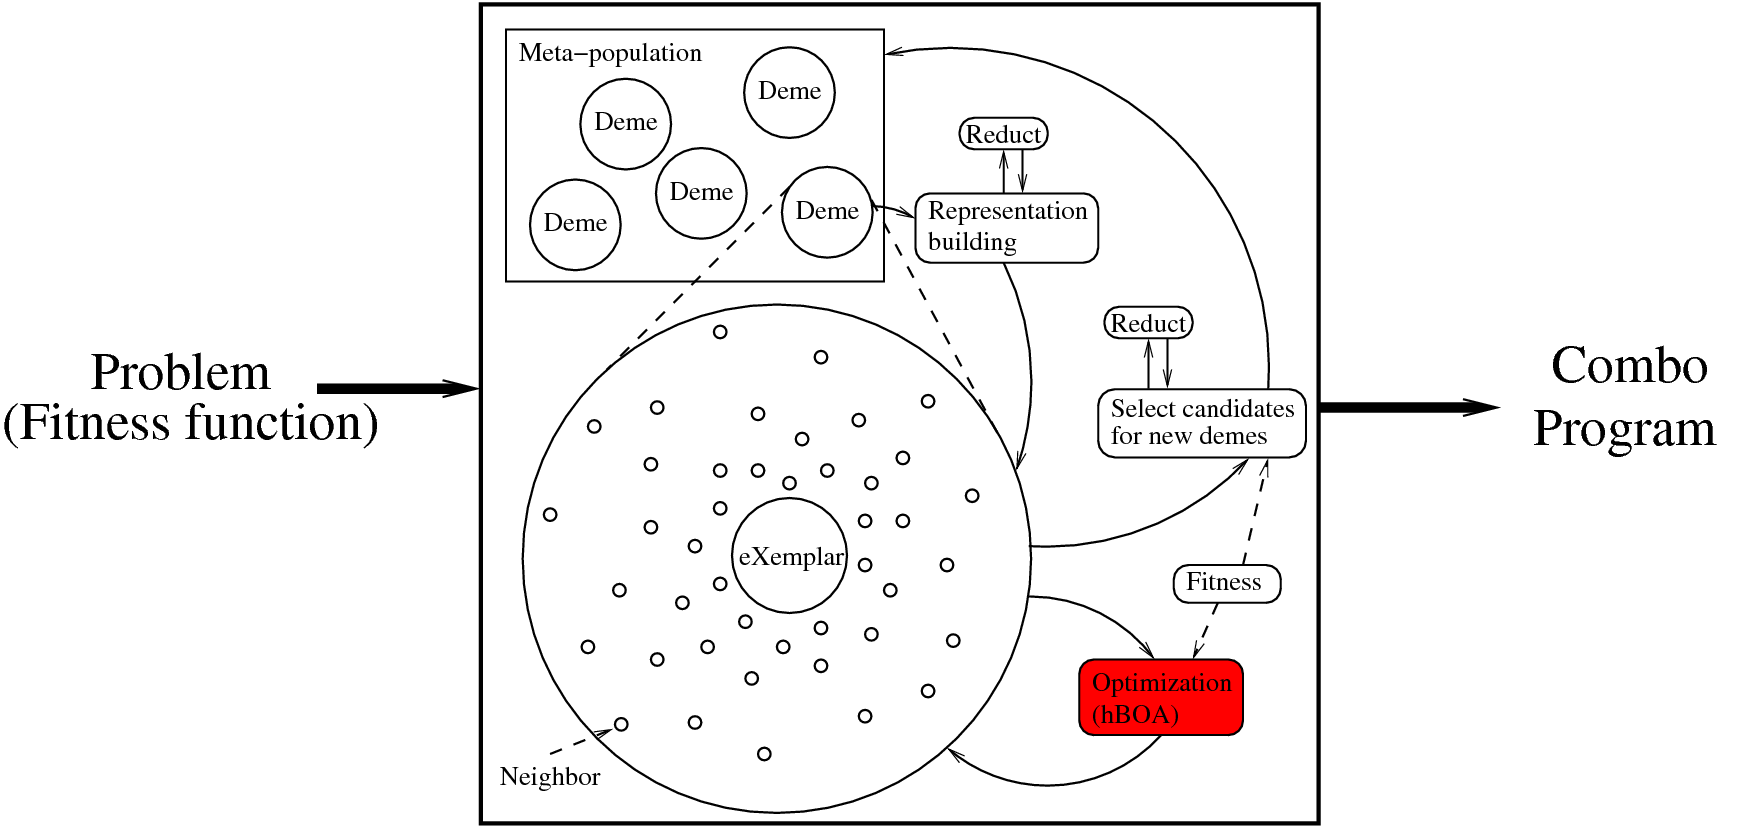
\includegraphics[scale=0.2]{MOSESSumDetailsO.png}

  \end{center}  
}

\frame
{
  \frametitle{MOSES' Optimization algorithms}

  \begin{enumerate}
  \item<+-> hBOA, multivariate model-building
    (not yet ported to the OpenCog version, univariate model-building instead)
  \item<+-> Hill-Climbing
  \item<+-> Building-Block Hill-Climbing (being ported to the OpenCog version)
  \end{enumerate}
}

\frame
{

  \frametitle{\emph{Hierarchical Bayesian Optimization Algorithm} (hBOA)}

  \begin{columns}

    \column{1.5in}

    $
    {\small
    \begin{array}{|c|c|}
      \hline
      Candidate & score \\
      \hline
      \only<1-5>{{\color<2->{yellow}00001010}}
      \only<6>{10011010}
      &
      \only<1-5>{{\color<2->{yellow}0.2}}
      \only<6>{0.5}
      \\
      \only<1-5>{{\color<2->{pink}00011010}}
      \only<6>{00111011}
      &
      \only<1-5>{{\color<2->{pink}0.6}}
      \only<6>{0.6}
      \\
      \only<1-5>{{\color<2->{yellow}01000100}}
      \only<6>{11111001}
      &
      \only<1-5>{{\color<2->{yellow}0.01}}
      \only<6>{0.7}
      \\
      \only<1-5>{{\color<2->{pink}00110110}}
      \only<6>{00111010}
      &
      \only<1-5>{{\color<2->{pink}0.5}}
      \only<6>{0.4}
      \\
      \only<1-5>{{\color<2->{pink}10010010}}
      \only<6>{10000001}
      &
      \only<1-5>{{\color<2->{pink}0.6}}
      \only<6>{0.1}
      \\
      $\vdots$ & $\vdots$\\
      \hline
    \end{array}
    }
    $
    \column{1.5in}

    \includegraphics[scale=0.25]<+>{population.png}
    \includegraphics[scale=0.25]<+>{good_vs_bad.png}
    \includegraphics[scale=0.25]<+>{good_vs_bad_class.png}
    \includegraphics[scale=0.25]<+>{good_vs_bad_prob_class.png}
%    \only<+>{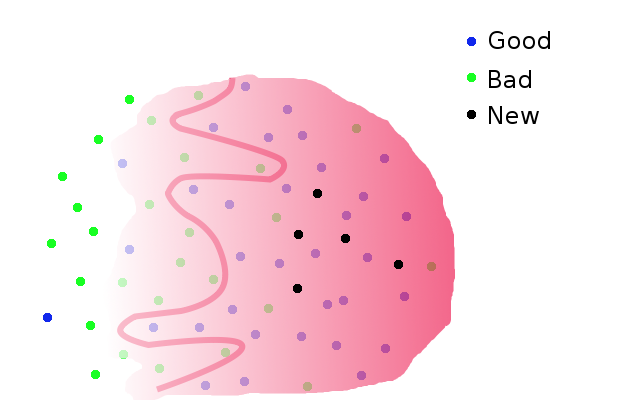
\includegraphics[scale=0.25]{good_vs_bad_new1.png}}
%    \only<+>{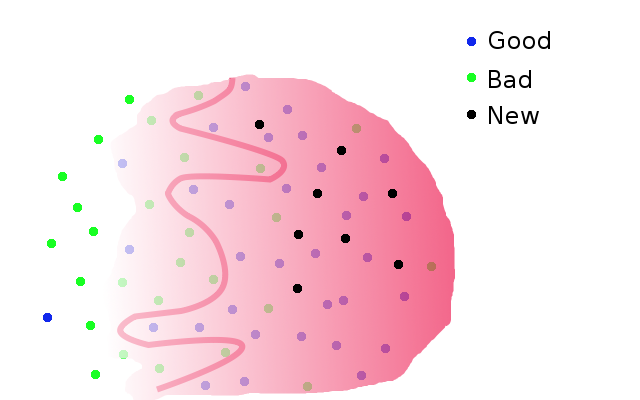
\includegraphics[scale=0.25]{good_vs_bad_new2.png}}
%    \only<+>{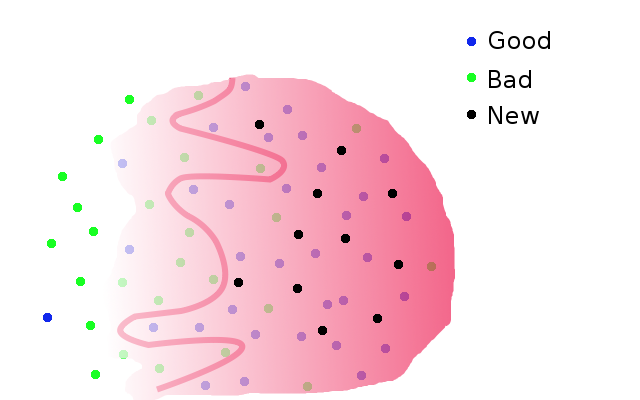
\includegraphics[scale=0.25]{good_vs_bad_new3.png}}
%    \only<+>{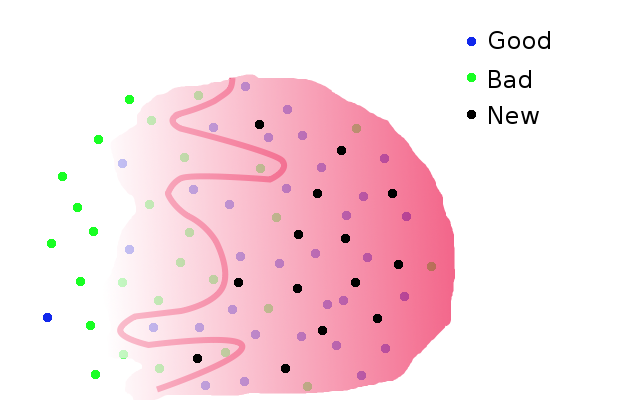
\includegraphics[scale=0.25]{good_vs_bad_new4.png}}
%    \only<+>{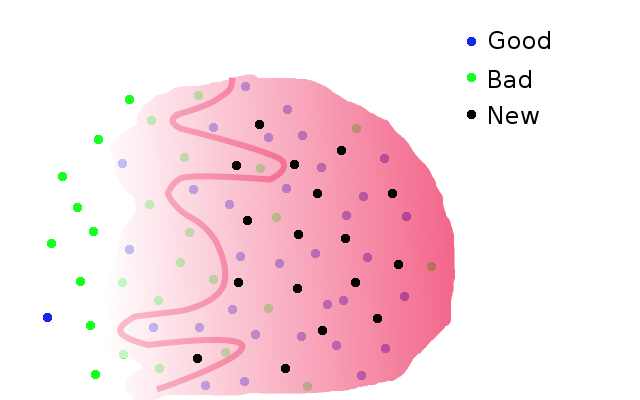
\includegraphics[scale=0.25]{good_vs_bad_new5.png}}
    \includegraphics[scale=0.25]<+>{good_vs_bad_new6.png}
    \includegraphics[scale=0.25]<+>{only_new.png}

%     \only<+>{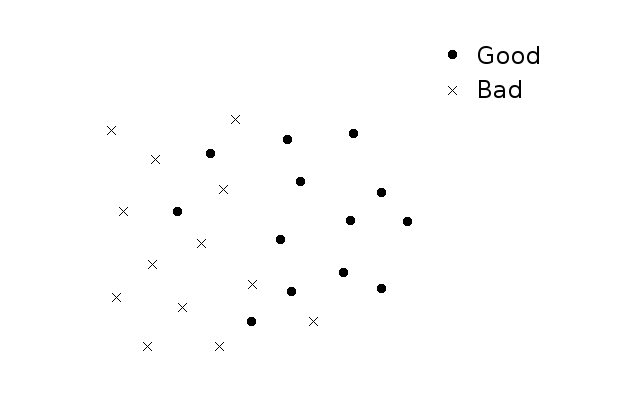
\includegraphics[scale=0.25]{GoodVsBad.png}}
%     \only<+>{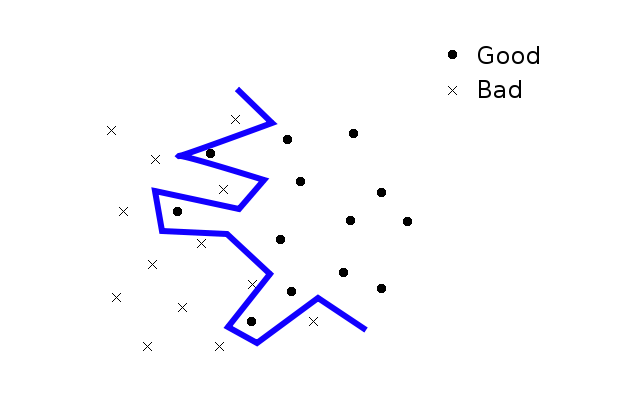
\includegraphics[scale=0.25]{GoodVsBadClass.png}}
%     \only<+>{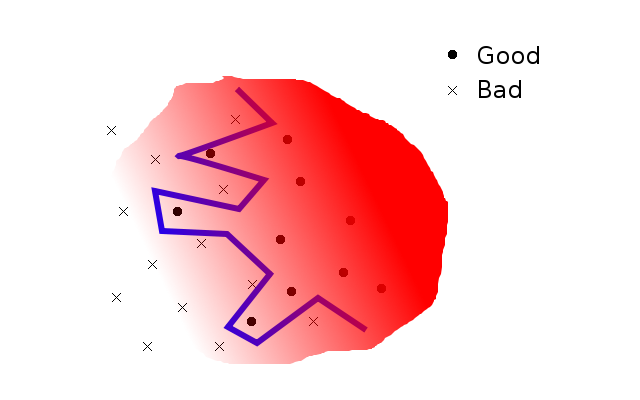
\includegraphics[scale=0.25]{GoodVsBadProbClass.png}}
%     \only<+>{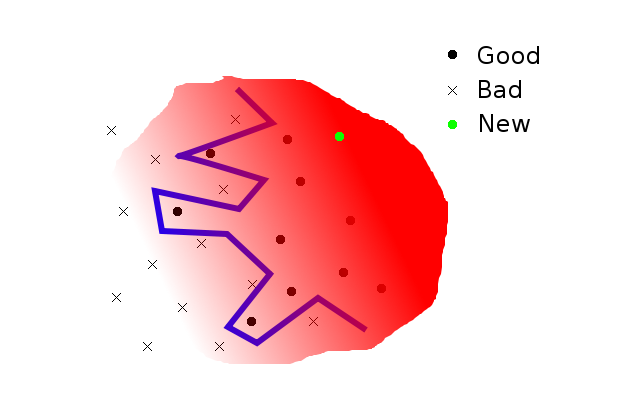
\includegraphics[scale=0.25]{GoodVsBadNewCand1.png}}
%     \only<+>{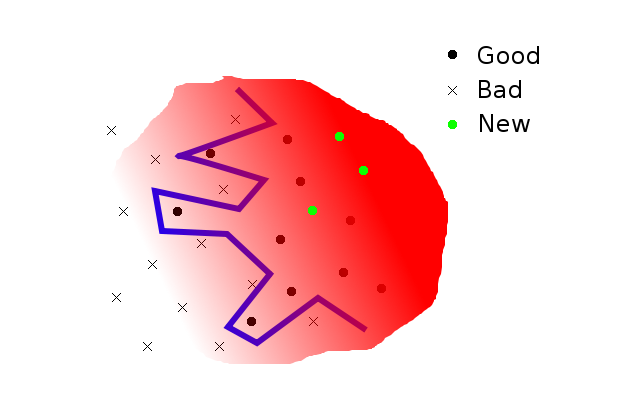
\includegraphics[scale=0.25]{GoodVsBadNewCand2.png}}
%     \only<+>{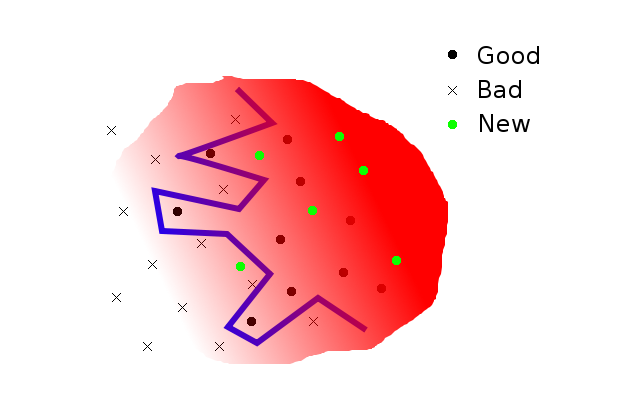
\includegraphics[scale=0.25]{GoodVsBadNewCand3.png}}
%     \only<+>{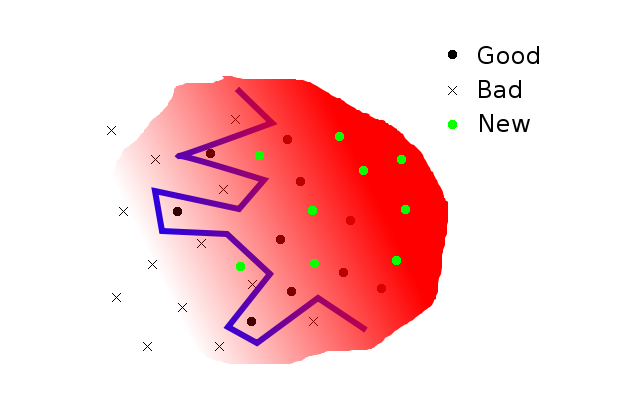
\includegraphics[scale=0.25]{GoodVsBadNewCand4.png}}
%     \only<+>{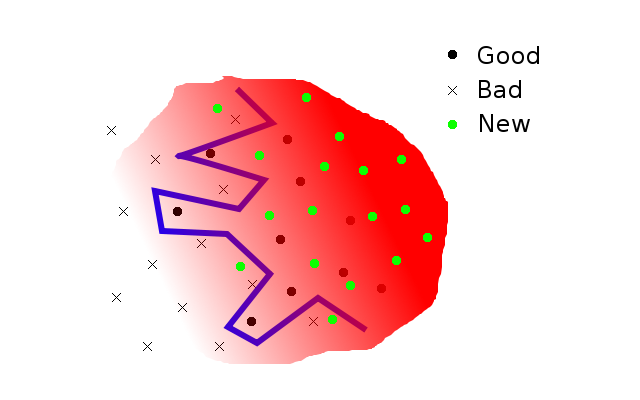
\includegraphics[scale=0.25]{GoodVsBadNewCand5.png}}
    
  \end{columns}

  \begin{itemize}
  \item<2-> Split the population in \alert{good vs bad candidates}
  \item<3-> \alert{Learn a classifier}, but not too strict or incorrect
  \item<4-> Probabilistic classifier,
    \alert{distribution of good candidates}
  \item<5-> \alert{Sample new candidates} according to the distribution
  \item<6-> Repeat on the new population
  \end{itemize}

}

\frame
{
  \frametitle{Distribution of Good Candidates: \alert{Bayesian Network}}

  \begin{columns}

    \column{1in}

    $
    {\small
    \begin{array}{|r|c|}
      \hline
      Candidate\ (X_i) & score \\
      i: 12345678 & \\
%      \hline
%      X_1 X_2 X_3 X_4 X_5 X_6 X_7 X_8 & \\
      \hline
      {\color{yellow}00001010}
      &
      {\color{yellow}0.2}
      \\
      {\color{pink}00011010}
      &
      {\color{pink}0.6}
      \\
      {\color{yellow}01000100}
      &
      {\color{yellow}0.01}
      \\
      {\color{pink}00110110}
      &
      {\color{pink}0.5}
      \\
      {\color{pink}10010010}
      &
      {\color{pink}0.6}
      \\
      \vdots & \vdots\\
      \hline
    \end{array}
    }
    $

    \column{2in}

%      $
%      {\small
%      \begin{array}{|c|c|c|c|c|c|c|c|}
%        \hline
%        X_1 & X_2 & X_3 & X_4 & X_5 & X_6 & X_7 & X_8 \\
%        \hline
%      \end{array}
%      }
%      $
%    \end{columns}

%    \pause

    %{\tiny
      \begin{tikzpicture}[node distance   = 1.4 cm]
        \GraphInit[vstyle=Shade]
        \tikzset{LabelStyle/.style =   {draw,
            fill  = yellow,
            text  = red}}
        \Vertex[L=$X_2$]{X2}
        \EA[L=$X_4$](X2){X4}
        \EA[L=$X_7$](X4){X7}
        \EA[L=$X_8$](X7){X8}
        \SO[L=$X_1$](X4){X1}
        \SOWE[L=$X_5$](X1){X5}
        \SOEA[L=$X_6$](X1){X6}
        \EA[L=$X_3$](X6){X3}
        \tikzset{EdgeStyle/.append style = {->}}
        \Edge(X7)(X8)
        \Edge(X1)(X5)
        \Edge(X1)(X6)
        \Edge(X5)(X6)
        \Edge(X6)(X3)
      \end{tikzpicture}
    %}

  \end{columns}

}

\frame
{
  \frametitle{Decomposing the problem into sub-problems}

  \begin{columns}

    \column{2in}

    \begin{tikzpicture}[node distance   = 1.4 cm]
      \GraphInit[vstyle=Shade]
      \tikzset{LabelStyle/.style =   {draw,
          fill  = yellow,
          text  = red}}
      \Vertex[L=$X_2$]{X2}
      \EA[L=$X_4$](X2){X4}
      \EA[L=$X_7$](X4){X7}
      \EA[L=$X_8$](X7){X8}
      \SO[L=$X_1$](X4){X1}
      \SOWE[L=$X_5$](X1){X5}
      \SOEA[L=$X_6$](X1){X6}
      \EA[L=$X_3$](X6){X3}
      \tikzset{EdgeStyle/.append style = {->}}
      \Edge(X7)(X8)
      \Edge(X1)(X5)
      \Edge(X1)(X6)
      \Edge(X5)(X6)
      \Edge(X6)(X3)
    \end{tikzpicture}

    \column{1.5in}
    \\[10ex]

    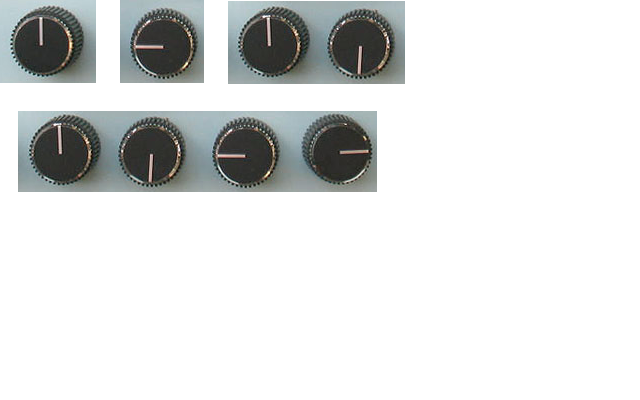
\includegraphics[scale=0.3]{knobs_problems.png}

  \end{columns}
}

\frame
{
  
  \frametitle{Conditional Probability with \alert{Decision Tree}}

  \begin{columns}

    \column{1in}

  $
  \begin{array}{|l|r|}
    \hline
    Marginal & Prob\\
    \hline
    P(X_1=1) & 0.3\\
    \hline
    P(X_2=1) & 0.05\\
    \hline
    P(X_4=1) & 0.9\\
    \hline
    P(X_7=1) & 0.88\\
    \hline
  \end{array}
  $

  \column{2in}
  
  $
  \begin{array}{|l|c|}
    \hline
    Conditional & Prob\\
    \hline
    P(X_8|X_7) &
    \text{\Tree [.$X_8$ $0.7$ [.$X_7$ $0.1$ $0.2$ ] ]} \\
    \hline
    P(X_5|X_1) & \ldots \\
    \hline
    P(X_6|X_1,X_5) & \ldots\\
    \hline
    P(X_3|X_6) & \ldots\\
    \hline
  \end{array}
  $

  \end{columns}

}

\frame
{  
  \frametitle{In OpenCog for the moment only \alert{univariate}}

  \begin{beamerboxesrounded}{Univariate}
    Only marginal probabilities
  \end{beamerboxesrounded}
  \begin{center}
  $
  \begin{array}{|l|r|}
    \hline
    Marginal & Prob\\
    \hline
    P(X_1=1) & 0.3\\
    \hline
    P(X_2=1) & 0.05\\
    \hline
    P(X_3=1) & 0.2\\
    \hline
    P(X_4=1) & 0.5\\
    \hline
    P(X_5=1) & 0.4\\
    \hline
    P(X_6=1) & 0.7\\
    \hline
    P(X_7=1) & 0.88\\
    \hline
    P(X_8=1) & 0.1\\
    \hline
  \end{array}
  $
  \end{center}

}

\frame
{
  \frametitle{Hill-Climbing, Building-Block Hill-Climbing}

  \begin{itemize}
  \item<+-> Hill-Climbing
    \begin{center}
      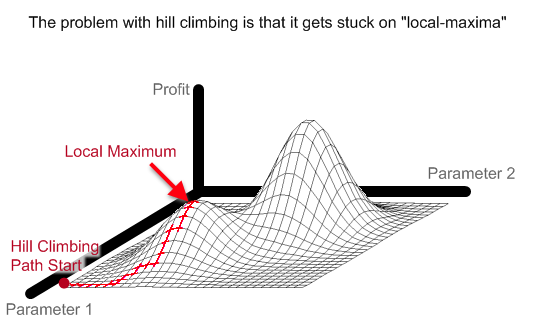
\includegraphics[scale=0.3]{HillClimbingLocalMax.png}
    \end{center}
  \item<+-> Building-Block Hill-Climbing $\Rightarrow$
    Redefine neighborhood to take short-cuts.
  \end{itemize}
  
}

\section{Deme management}

\frame{

  \frametitle{Select Candidates for Future Demes}

  \begin{center}
    
    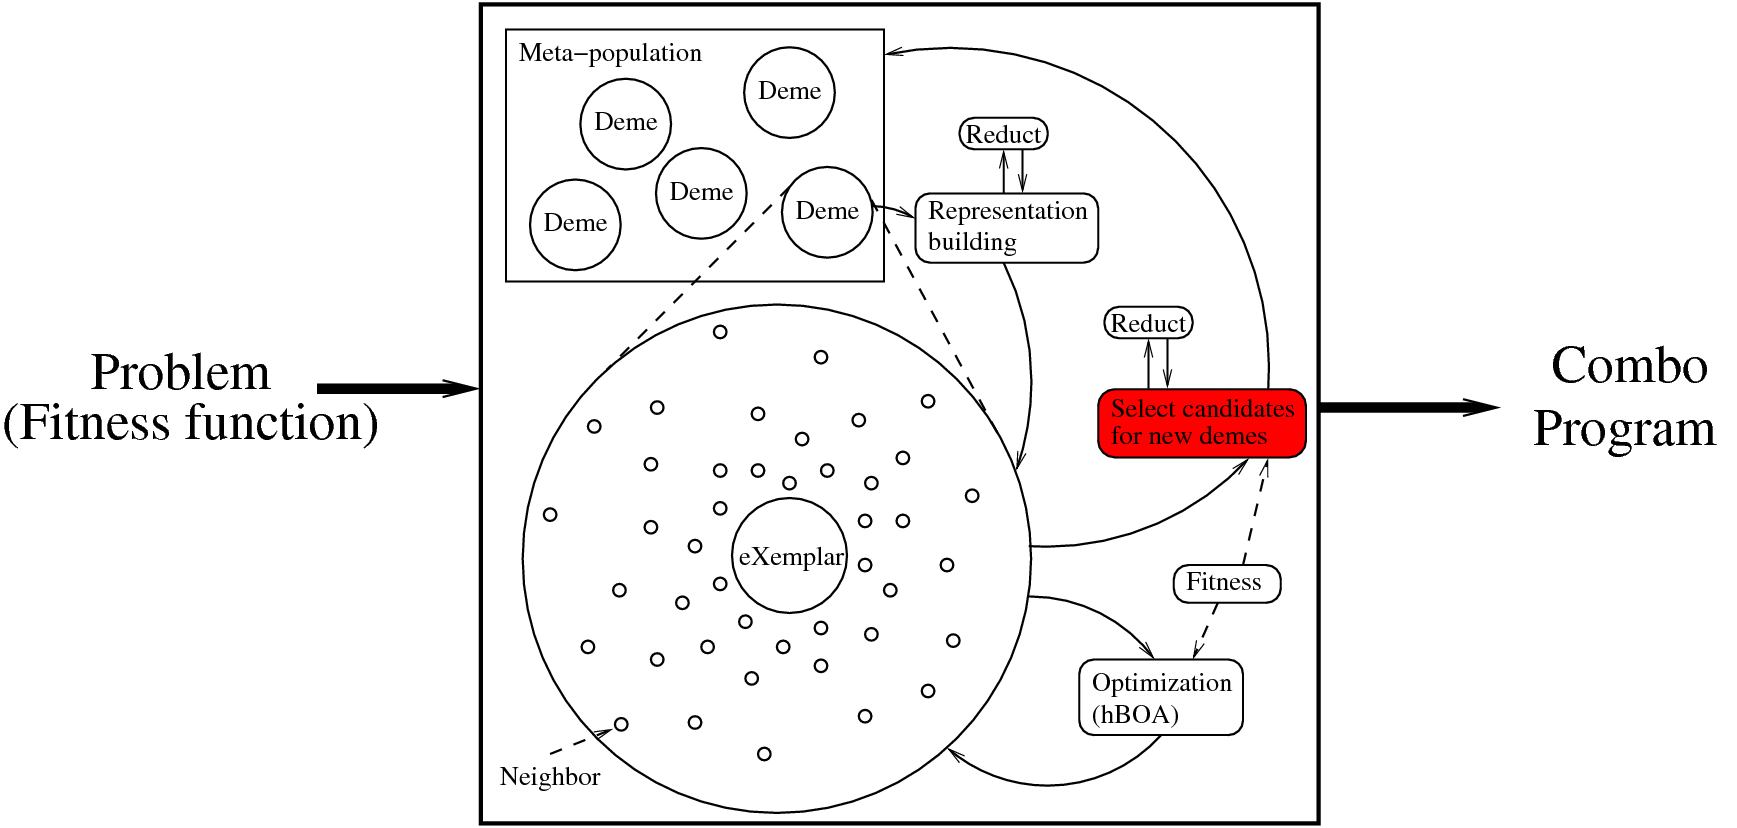
\includegraphics[scale=0.2]{MOSESSumDetailsSC.png}

  \end{center}  
}

\frame
{
  \frametitle{Preserving Diversity, 
    candidates that behave differently and non-dominated}

  \pause


  \begin{center}

    \visible<5->{
      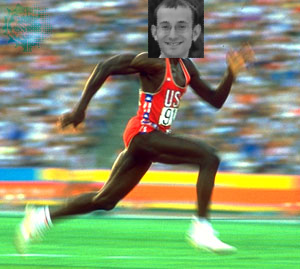
\includegraphics[scale=0.2]{MosheLewis.png}
    }

  \end{center}

  \begin{columns}
    
    \column{0.5in}

    \column{1in}

    \visible<2->{
        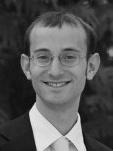
\includegraphics[scale=0.4]{moshe_head_bw.jpg}
    }
    \column{1.5in}
    
    \visible<3->{
        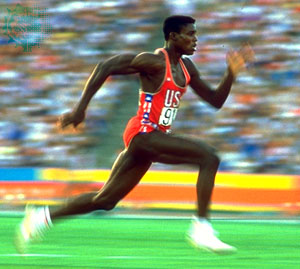
\includegraphics[scale=0.2]{CarlLewis2.jpg}
    }
  \end{columns}

  \begin{itemize}
  \item<4-> Neither one dominates the other
  \item<5-> But ``Moshe Lewis'' dominates then both
  \end{itemize}
}  

\frame
{
  \frametitle{Behavioral score}

  \begin{beamerboxesrounded}{Behavioral score}
    Partial order
    \begin{itemize}
    \item<+-> if c1 < c2 then \alert{c1 is dominated by c2}
    \item<+-> if c1 > c2 then \alert{c1 dominates c2}
    \item<+-> otherwise,
      \alert{neither one dominates the other}
    \end{itemize}
  \end{beamerboxesrounded}
  \pause
  For instance: \alert{vector of floats}
  $(f_1, \ldots , f_n)$ where each
  $f_i$ measure how well a candidate is doing for that particular feature.

  If for all features $i$,
  $c1$ is doing better than $c2$, then $c1$ dominates $c2$.
}

%\frame
%{
%  OR(AND(#1 #2) AND(NOT(#1) NOT(#2)))
%}

\frame
{ 
  \begin{beamerboxesrounded}{Deme selection}
    Keep non-dominated exemplars as potential deme.
  \end{beamerboxesrounded}

  \pause
  We want to \alert{learn $f(x)$}.


  \only<1,2>{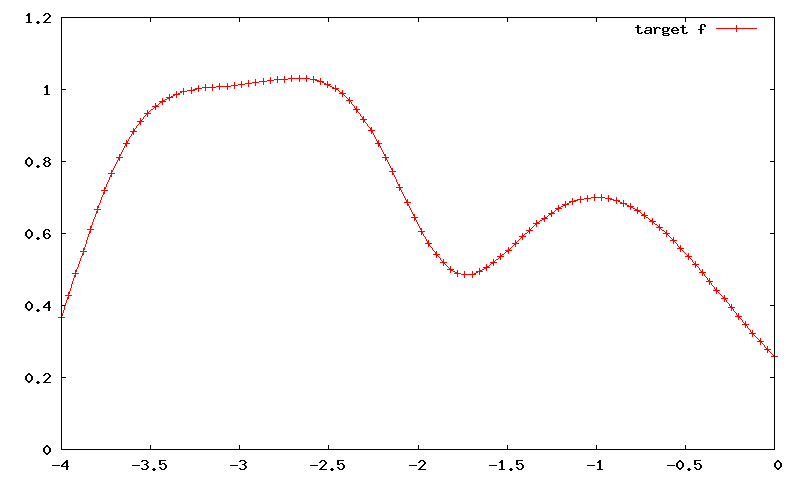
\includegraphics[scale=0.25]{domine.png}}
  \only<3>{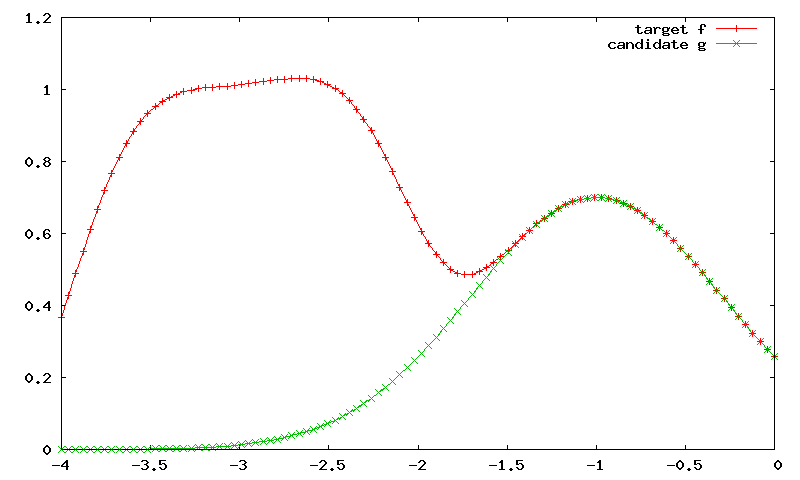
\includegraphics[scale=0.25]{domine2.png}}
  \only<4>{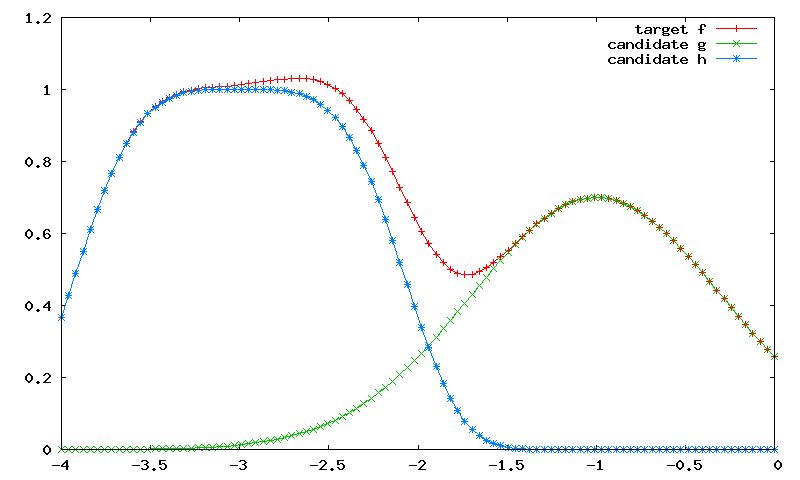
\includegraphics[scale=0.25]{domine3.png}}
  \only<5->{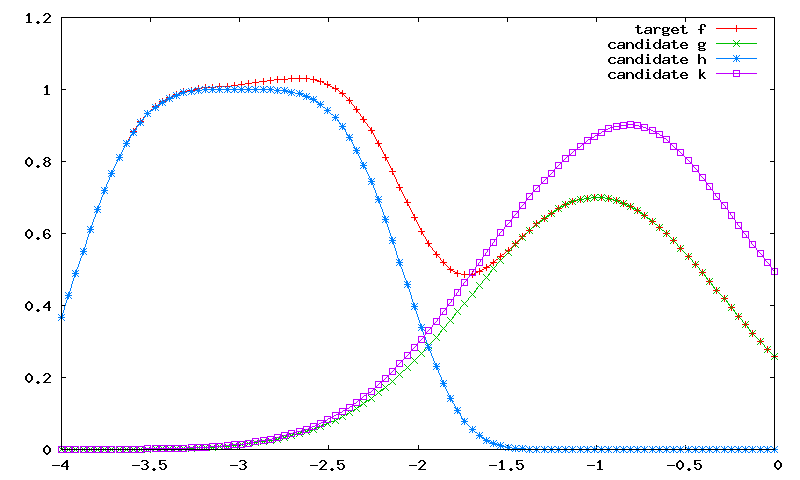
\includegraphics[scale=0.25]{domine4.png}}

  \visible<6>{
    \alert{$k(x)$ is dominates by $g(x)$}
      and will not be included in the meta-population}

}

\frame
{
  \begin{center}

  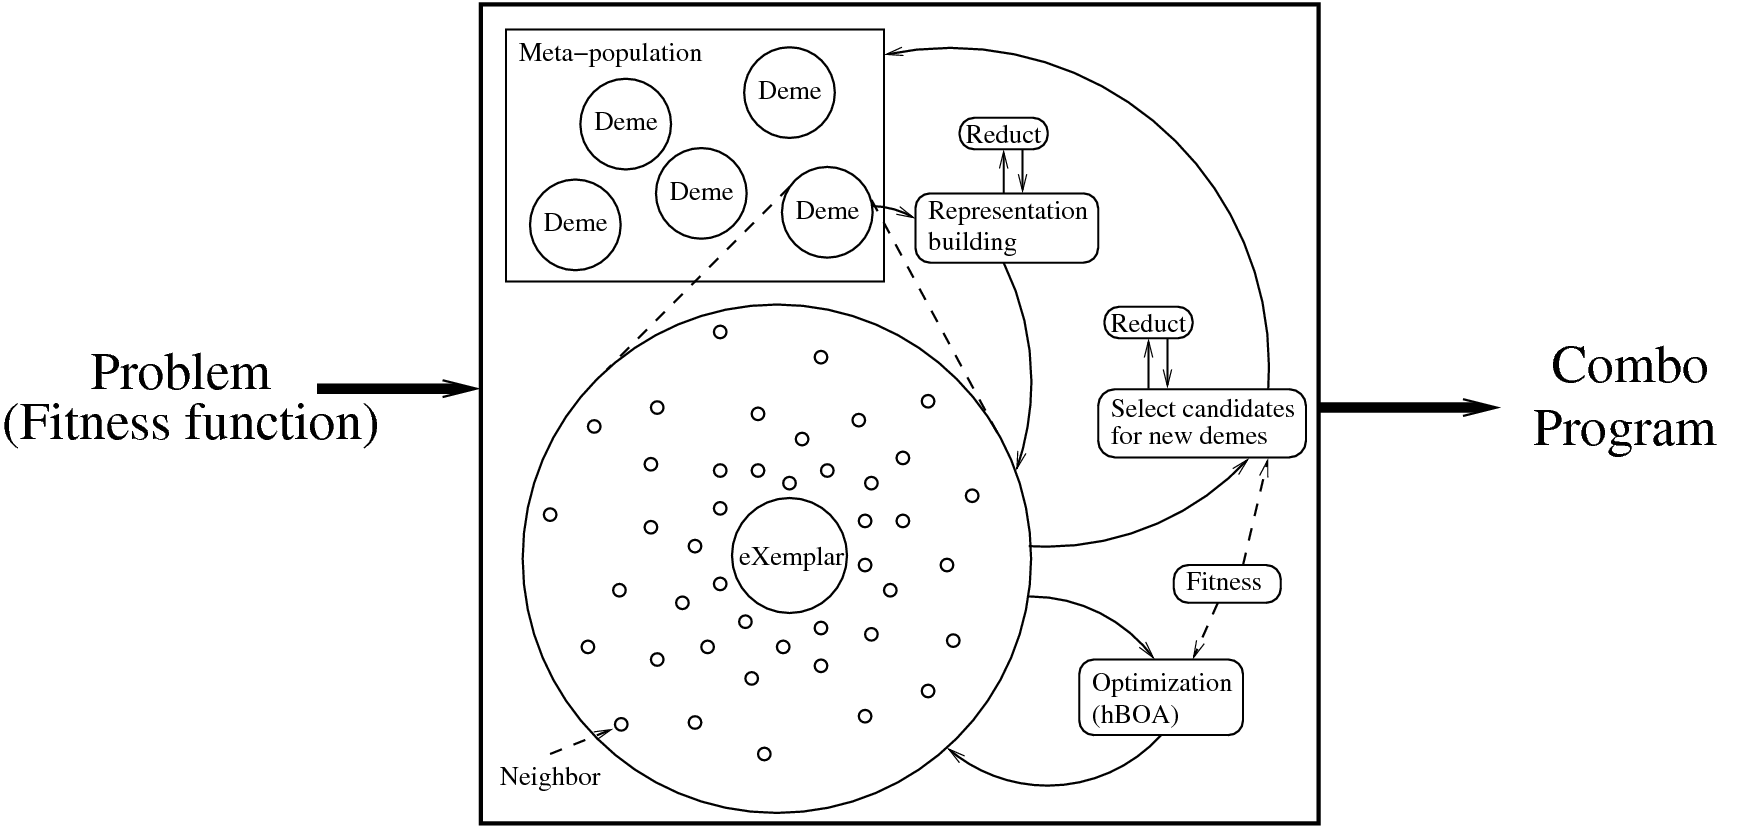
\includegraphics[scale=0.2]{MOSESSumDetails.png}

  \end{center}
}

\frame
{
  \frametitle{Some benchmark}
  \begin{center}
    \begin{figure}
      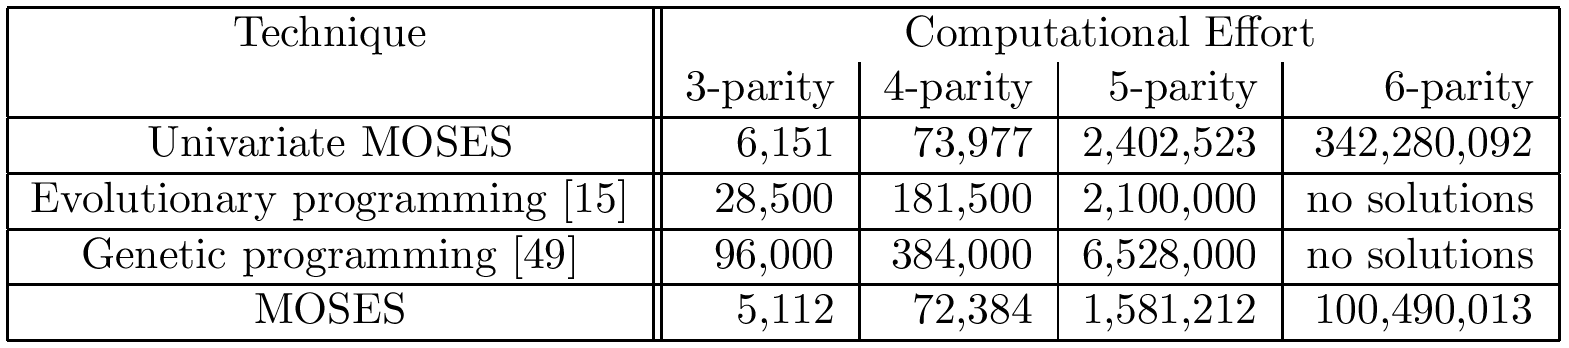
\includegraphics[scale=0.25]{benchmark.png}
      \caption{Computational effort to find solution of n-parity 99\%
        of the time \emph{(extracted from Moshe's PhD thesis)}}
    \end{figure}
  \end{center}
  \[{\text {\it n-parity}}(b_1, \ldots, b_n) =
  {\it even}\left(\sum_{i=1}^n int(b_i)\right)\]
}
\section{Demo...}

\section{Conclusion}

\frame
{
  \frametitle{Conclusion}

  MOSES outperforms Genetic Algorithms because:
   \begin{enumerate}
   \item<+-> minimize over-representation (\alert{Reduction in normal form})
   \item<+-> build expressive deme population by taking into account
     operator semantics (\alert{representation-building})
   \item<+-> Maintain diversity in the meta-population (\alert{deme managment})
   \item<+-> Attempt to find regularities in one deme's population to
     speed up optimization (\alert{model-building})
   \end{enumerate}
}

\frame
{
  \frametitle{What remains to be done?}

  \begin{enumerate}
  \item<+-> Only handles Boolean, continuous, numerico-boolean and
    (partially) action-perception expressions\\
    $\Rightarrow$ \alert{more programmatic construct}
  \item<+-> Representation-building is hard-coded per operator set\\
    $\Rightarrow$ Generalized for \alert{operator properties
      (especially useful if combined with PLEASURE)}
  \item<+-> Model-building is slow\\
    $\Rightarrow$ \alert{improve model-building} (better Bayesian learning,
    transfer learning across populations), or use other optimization method
  \item<+-> No transfer learning across problem instances\\
    $\Rightarrow$ Integrative AGI, Attention Allocation, PLN, etc.
  \end{enumerate}
}

\end{document}
